\documentclass[border=6pt]{standalone}
% Match the user-provided correctness TikZ reference: Computer Modern Sans,
% normalsize node text and scriptsize annotations. All weights remain regular
% per the user preference; do not copy the reference textbf wrappers.
% Horizontal spacing accommodates the larger/heavier labels.
\usepackage{tikz}
\usetikzlibrary{arrows.meta,positioning,calc,fit,backgrounds}
% Exact paper palette: shared correctness colours from diagrams/correctness_detail.tex;
% translation/optimization colours from diagrams/overall_architecture.tex.
\definecolor{trans}{RGB}{106,61,154}
\definecolor{transfill}{RGB}{233,223,245}
\definecolor{opt}{RGB}{55,71,133}
\definecolor{optfill}{RGB}{224,229,247}
\definecolor{corr}{RGB}{13,110,100}
\definecolor{corrfill}{RGB}{206,235,231}
\definecolor{gold}{RGB}{150,110,6}
\definecolor{goldfill}{RGB}{250,232,186}
\definecolor{retry}{RGB}{176,34,34}
\begin{document}
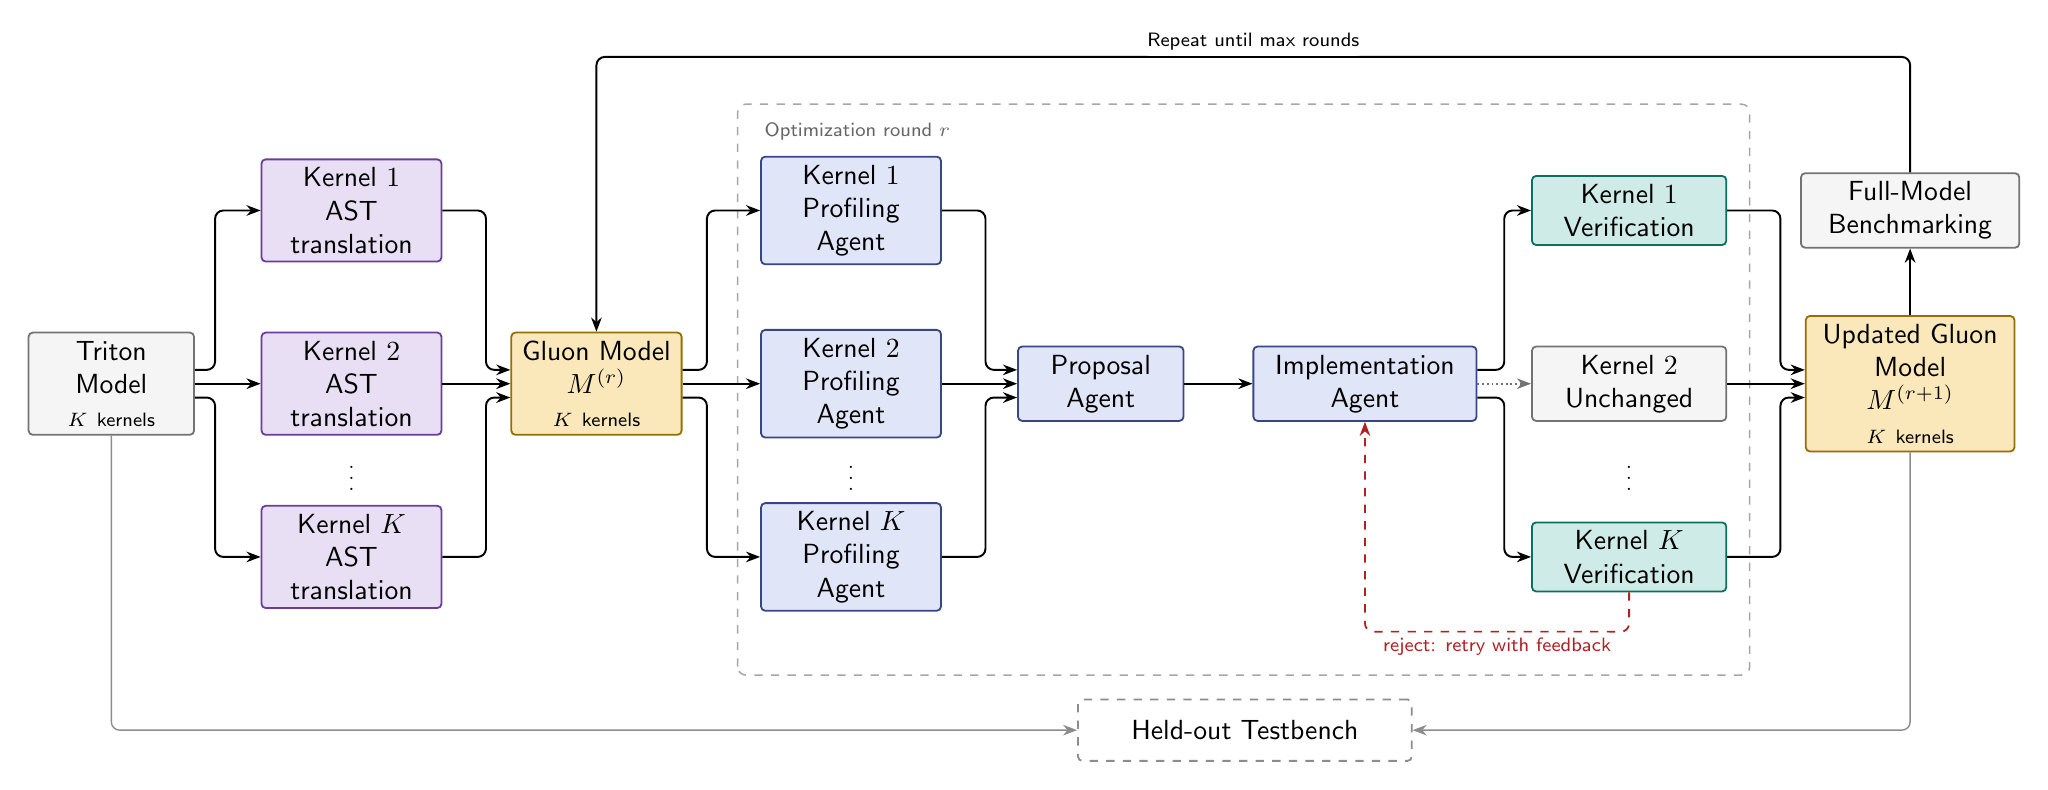
\begin{tikzpicture}[
 x=1.22cm, font=\sffamily, >=Stealth,
 box/.style={draw=black!55,fill=white,line width=.65pt,rounded corners=1.5pt,
 align=center,minimum height=.78cm,inner sep=3pt,text width=1.647cm,font=\sffamily\mdseries\normalsize},
 model/.style={box,draw=gold,fill=goldfill,font=\sffamily\mdseries\normalsize},
 source/.style={box,fill=black!4,font=\sffamily\mdseries\normalsize},
 trans/.style={box,draw=trans,fill=transfill},
 opt/.style={box,draw=opt,fill=optfill},
 corr/.style={box,draw=corr,fill=corrfill},
 bench/.style={box,fill=black!4},
 test/.style={box,draw=black!45,dashed,text width=4.026cm},
 a/.style={-{Stealth[length=1.8mm]},line width=.7pt,rounded corners=3pt},
 wire/.style={line width=.7pt,rounded corners=3pt},
 carry/.style={a,densely dotted,draw=black!55},
 reject/.style={a,dashed,draw=retry,line width=.65pt},
 eval/.style={a,draw=black!45,line width=.5pt},
 tag/.style={font=\sffamily\scriptsize,fill=white,inner sep=2pt,align=center},
 phase/.style={font=\sffamily\mdseries\scriptsize,text=black!60},
 frame/.style={draw=black!35,dashed,rounded corners=3pt,line width=.55pt}
]

\node[source,text width=1.891cm] (src) at (0,0) {Triton Model\\{\scriptsize $K$ kernels}};
\node[model,text width=1.952cm] (state) at (5.05,0) {Gluon Model\\$M^{(r)}$\\{\scriptsize $K$ kernels}};
\node[opt,text width=1.891cm] (prop) at (10.3,0) {Proposal\\Agent};
\node[opt,text width=2.623cm] (impl) at (13.05,0) {Implementation\\Agent};
\node[model,text width=2.440cm] (next) at (18.725,0) {Updated Gluon\\Model\\$M^{(r+1)}$\\{\scriptsize $K$ kernels}};
\node[bench,text width=2.562cm] (bench) at (18.725,2.2) {Full-Model\\Benchmarking};
\node[trans,text width=2.074cm] (a1) at (2.5,2.2) {Kernel $1$\\AST translation};
\node[opt,text width=2.074cm] (p1) at (7.7,2.2) {Kernel $1$\\Profiling Agent};
\draw[a] ([yshift=5pt]src.east) -- (1.08,0.17573) |- (a1.west);
\draw[a] (a1.east) -- (3.9,2.2) |- ([yshift=5pt]state.west);
\draw[a] ([yshift=5pt]state.east) -- (6.2,0.17573) |- (p1.west);
\draw[a] (p1.east) -- (9.1,2.2) |- ([yshift=5pt]prop.west);
\node[corr,text width=2.257cm] (v1) at (15.8,2.2) {Kernel $1$\\Verification};
\draw[a,rounded corners=3pt] ([yshift=5pt]impl.east) -- (14.5,0.17573) |- (v1.west);
\draw[a] (v1.east) -- (17.375,2.2) |- ([yshift=5pt]next.west);
\node[trans,text width=2.074cm] (a2) at (2.5,0) {Kernel $2$\\AST translation};
\node[opt,text width=2.074cm] (p2) at (7.7,0) {Kernel $2$\\Profiling Agent};
\draw[a] (src.east) -- (a2.west);
\draw[a] (a2.east) -- (state.west);
\draw[a] (state.east) -- (p2.west);
\draw[a] (p2.east) -- (prop.west);
\node[trans,text width=2.074cm] (a3) at (2.5,-2.2) {Kernel $K$\\AST translation};
\node[opt,text width=2.074cm] (p3) at (7.7,-2.2) {Kernel $K$\\Profiling Agent};
\draw[a] ([yshift=-5pt]src.east) -- (1.08,-0.17573) |- (a3.west);
\draw[a] (a3.east) -- (3.9,-2.2) |- ([yshift=-5pt]state.west);
\draw[a] ([yshift=-5pt]state.east) -- (6.2,-0.17573) |- (p3.west);
\draw[a] (p3.east) -- (9.1,-2.2) |- ([yshift=-5pt]prop.west);
\node[corr,text width=2.257cm] (v3) at (15.8,-2.2) {Kernel $K$\\Verification};
\draw[a,rounded corners=3pt] ([yshift=-5pt]impl.east) -- (14.5,-0.17573) |- (v3.west);
\draw[a] (v3.east) -- (17.375,-2.2) |- ([yshift=-5pt]next.west);
\draw[a] (prop) -- (impl);
\draw[a] (next.north) -- (bench.south);
\node[box,fill=black!4,text width=2.257cm] (u2) at (15.8,0) {Kernel $2$\\Unchanged};
\draw[carry] (impl.east) -- (u2.west);
\draw[a] (u2.east) -- (next.west);
\draw[reject] (v3.south) -- (15.8,-3.15) -- node[tag,below,text=retry] {reject: retry with feedback} (13.05,-3.15) -- (impl.south);
\node[font=\scriptsize,inner sep=0pt] at (2.5,-1.1) {$\vdots$};
\node[font=\scriptsize,inner sep=0pt] at (7.7,-1.1) {$\vdots$};
\node[font=\scriptsize,inner sep=0pt] at (15.8,-1.1) {$\vdots$};
\begin{scope}[on background layer]\draw[frame] (6.52,-3.70) rectangle (17.055,3.55);\end{scope}
\node[phase,anchor=north west] at (6.7,3.43) {Optimization round $r$};
\draw[a] (bench.north) -- (18.725,4.15) -- node[tag,above] {Repeat until max rounds} (5.05,4.15) -- (state.north);
\node[test] (test) at (11.8,-4.4) {Held-out Testbench};
\draw[eval] (src.south) |- (test.west);
\draw[eval] (next.south) |- (test.east);

\end{tikzpicture}
\end{document}
